

This section begins with discussion of further autoinducers and antibiotics which could be used in future conjugates. 
Some have have already been partially or fully synthesised by myself or other members of the Spring group.
Plans for further biological testing of the conjugates synthesised in this study are then presented.

\subsubsection{Autoinducer derivatives}

\subsubsubsection{3-oxo-C$_{12}$-HSL derivative \compound{cmpd:HLO12N3} \label{sec:Fut_HLO12}}

N$_3$-3-oxo-C$_{12}$-HSL \compound{cmpd:HLO12N3} (see \ref{sch:HLO12N3_synth}) was synthesised by Ryan Howard, a master's student under my supervision. The synthesis was based on a synthesis of 3-oxo-C$_{12}$-HSL \compound{cmpd:HLO12} reported by Hodgkinson \textit{et al.}\cite{Hodgkinson2011}. 
Conjugates of this compound were not included in the library as it degraded during the click reaction. However, reaction conditions could be further optimised, or the acetal-protected azide \compound{cmpd:HLac12N3} could be used in the click reaction, followed by deprotection.

This compound would be a useful addition to the library as it would demonstrate whether the 3-oxo group and/or longer alkyl chain are required for activity. As the head group is added fairly late in the synthesis it would also be easy to swap it for the other head groups described in \ref{sec:HSLCipCs}, thus expanding the library further.

\begin{scheme}[H]
	\begin{center}
		\schemeref[HO10Br]{cmpd:HO10Br}
		\schemeref[HO10N3]{cmpd:HO10N3}
		\schemeref[Cl10N3]{cmpd:Cl10N3}
		\schemeref[MeOO12N3]{cmpd:MeOO12N3}
		\schemeref[MeOac12N3]{cmpd:MeOac12N3}
		\schemeref[HOac12N3]{cmpd:HOac12N3}
		\schemeref[HLHBr]{cmpd:HLHBr}
		\schemeref[HLac12N3]{cmpd:HLac12N3}
		\schemeref[HLO12N3]{cmpd:HLO12N3}
		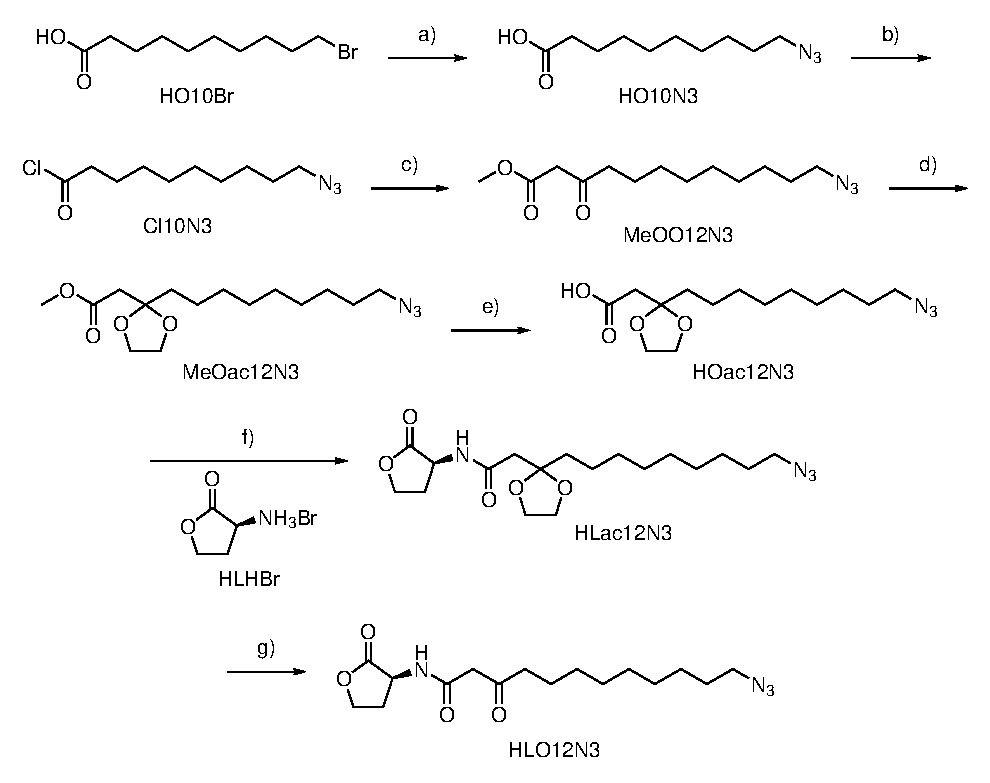
\includegraphics[scale=1]{HLO12N3_synth}
		\caption{The synthesis of N$_3$-3-oxo-C$_{12}$-HSL \compound{cmpd:HLO12N3} carried out by Ryan Howard.
		a) \ce{NaN3}, DMF, 60 $^{\circ}$C, 6 h, 93\%.
		b) Oxalyl chloride, DMF, \ce{CH2Cl2}, 3 h, r.t..
		c) MeOAc, \textit{N}-methyl imidazole, \ce{TiCl4}, DIPEA, toluene, r.t., 2 h, 43\% over two steps.
		d) \ce{HO(CH2)2OH}, TsOH, \ce{CH(OMe)3}, r.t., 5 h, 78\%.
		e) NaOH, water, r.t., 6 h, 85\%.
		f) EDC, DMAP, \ce{CH2Cl2}, r.t., 16 h.
		g) TFA, r.t., 5 h, 29\% over two steps.
		\label{sch:HLO12N3_synth}}
	\end{center}
\end{scheme}

\subsubsubsection{AI-2 derivatives}

AI-2 \compound{cmpd:AI2} is perhaps a more attractive choice of autoinducer for inclusion in conjugates than the others used in this study as it is actively transported into cells\cite{Taga2003} and used by a wide range of bacterial species\cite{Pereira2013}.
The synthesis of conjugates of AI-2 \compound{cmpd:AI2} with ciprofloxacin \compound{cmpd:Cip} and trimethoprim \compound{cmpd:Tri} has been attempted in the Spring group by Dr Jamie Stokes. However, the protected azido AI-2 derivative \compound{cmpd:AI2_J} synthesised was found to be unstable, and the click reactions attempted were unsuccessful\cite{Stokes2017}. AI-2 \compound{cmpd:AI2} is known to interconvert between multiple forms (including forming a furanosyl borate diester)\cite{Guo2015} so it is to be expected that syntheses involving it might be challenging. If a more stable azido AI-2\compound{cmpd:AI2} derivative cannot be developed, another approach would be to use an azido AI-2 \compound{cmpd:AI2} analogue which is capable of being taken up by the same active transport mechanism. 

\begin{figure}[H]
	\begin{center}
		\schemeref[AI2]{cmpd:AI2}
		\schemeref[AI2J]{cmpd:AI2_J}
		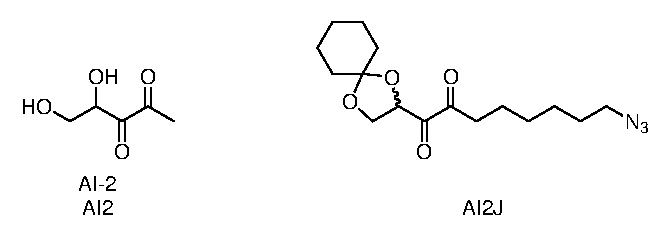
\includegraphics[scale=1]{AI2}
		\caption{AI-2 \compound{cmpd:AI2} in its DPD form and the protected azido AI-2 derivative \compound{cmpd:AI2_J} synthesised by Dr Jamie Stokes\cite{Stokes2017}.
		\label{fgr:AI2}} 
	\end{center}
\end{figure}

Two types of AI-2 \compound{cmpd:AI2} receptors have been identified: LuxP, present in \textit{Vibrio} spp.\cite{Chen2002}, and LsrB, first discovered in \textit{Salmonella enterica} serovar Typhimurium\cite{Miller2004}. 
LuxP is a periplasmic binding protein that relays the signal, but not the actual AI-2 \compound{cmpd:AI2} molecule, into the cell and hence is not a useful target.\cite{Neiditch2005}
LsrB is the ligand binding protein of a system that transports AI-2 \compound{cmpd:AI2} into the cell\cite{Taga2003}, and hence can be targeted. LsrB orthologs are found in a wide range of bacterial families including \textit{Enterobacteriaceae}, \textit{Rhizobiaceae}, and \textit{Bacillaceae}\cite{Pereira2009}.
In addition, several bacterial species, including \textit{P. aeruginosa}, are known to respond to AI-2 \compound{cmpd:AI2} but do not have either of these two known types of receptors, and thus the discovery of new receptor types is expected\cite{Pereira2009}. Any postulated receptor would need to internalise the AI-2 analogue in order for conjugates to be effective against the bacterium.

One example of an AI-2 analogue which could be derivatised is a geminal dibromo compound \compound{cmpd:PrAI2DBr} synthesised by Guo \textit{et al.}\cite{Guo2015} (see \ref{fgr:PrAI2DBr}). It is as potent as AI-2 at dissociating the LsrR repressor from the promotor region in a reporter strain, and may be more stable. It is also esterified, making it less volatile and thus easily purified using column chromatography. The esters are presumably cleaved by cellular esterases as the compounds can be used in QS assays without deprotection\cite{Guo2012}.

A possible azido derivative \compound{cmpd:PrAI2DBrN3} of this analogue is shown in \ref{fgr:PrAI2DBr}. If a route to it could be found, it appears to be a promising partner in future conjugates given the known properties of AI-2 \compound{cmpd:AI2}.

\begin{figure}[H]
	\begin{center}
		\schemeref[PrAI2DBr]{cmpd:PrAI2DBr}
		\schemeref[PrAI2DBrN3]{cmpd:PrAI2DBrN3}
		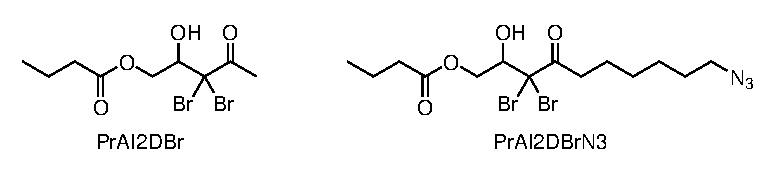
\includegraphics[scale=1]{PrAI2DBr}
		\caption{An AI-2 analogue \compound{cmpd:PrAI2DBr} synthesised by Guo \textit{et al.} and the proposed azido AI-2 analogue derivative \compound{cmpd:PrAI2DBrN3}.
		\label{fgr:PrAI2DBr}} 
	\end{center}
\end{figure}


%ComX and AIP are not transported into cells



\subsubsection{Antibiotic derivatives}

\subsubsubsection{Ciprofloxacin derivative \compound{cmpd:pipciphex}}

A second alkynyl ciprofloxacin derivative \compound{cmpd:pipciphex} was planned and partially synthesised during this project, and finishing this synthesis would provide a useful intermediate for future conjugates.

The derivative \compound{cmpd:pipciphex} has an alkyne tail attached in place of the cyclopropane ring as it has been shown that bulkier groups in this position can be tolerated\cite{Mitscher1986,Chu1985}. This synthesis followed a conventional route to ciprofloxacin \compound{cmpd:Cip} similar to that reported by Mitscher \textit{et al.}\cite{Mitscher1986} but used hex-5-yn-1-amine \compound{cmpd:hexam} instead of cyclopropylamine.

The \ce{TiCl4}-catalysed crossed Claisen condensation of the acid chloride \compound{cmpd:24Cl5FbCl} and ethyl acetate described by Hashimoto \textit{et al.} \cite{Hashimoto2006} was used to produce the $\beta$-ketoester.
The ethoxymethylene group in \compound{cmpd:24Cl5Fbkee} was installed by the reaction of $\beta$-ketoester \compound{cmpd:24Cl5Fbke} and triethyl orthoformate to give a mixture of the \textit{E} and \textit{Z} isomers\cite{Senthilkumar2009,Mitscher1986}.
Hex-5-yn-1-amine \compound{cmpd:hexam} was prepared using a Gabriel synthesis \cite{Gabriel1887} described by Rożkiewicz \textit{et al.} \cite{Rozkiewicz2006}. Unfortunately the amine was surprisingly volatile and was lost on evaporation of the reaction solvent. If a better purification method could be found, or a longer-chain alkynyl amine was used, the rest of the synthesis could be performed and the resulting alkynyl ciprofloxacin derivative \compound{cmpd:pipciphex} could be used to form more triazole-linked conjugates.

\begin{scheme}[H]
	\begin{center}
		\schemeref[24Cl5FbCl]{cmpd:24Cl5FbCl}
		\schemeref[24Cl5Fbke]{cmpd:24Cl5Fbke}
		\schemeref[24Cl5Fbket]{cmpd:24Cl5Fbket}
		\schemeref[24Cl5Fbkee]{cmpd:24Cl5Fbkee}
		\schemeref[hexCl]{cmpd:hexCl}
		\schemeref[hexphth]{cmpd:hexphth}
		\schemeref[hexam]{cmpd:hexam}
		\schemeref[24Cl5Fbkeam]{cmpd:24Cl5Fbkeam}
		\schemeref[ClciphexEt]{cmpd:ClciphexEt}
		\schemeref[Clciphex]{cmpd:Clciphex}
		\schemeref[pip]{cmpd:pip}
		\schemeref[pipciphex]{cmpd:pipciphex}
		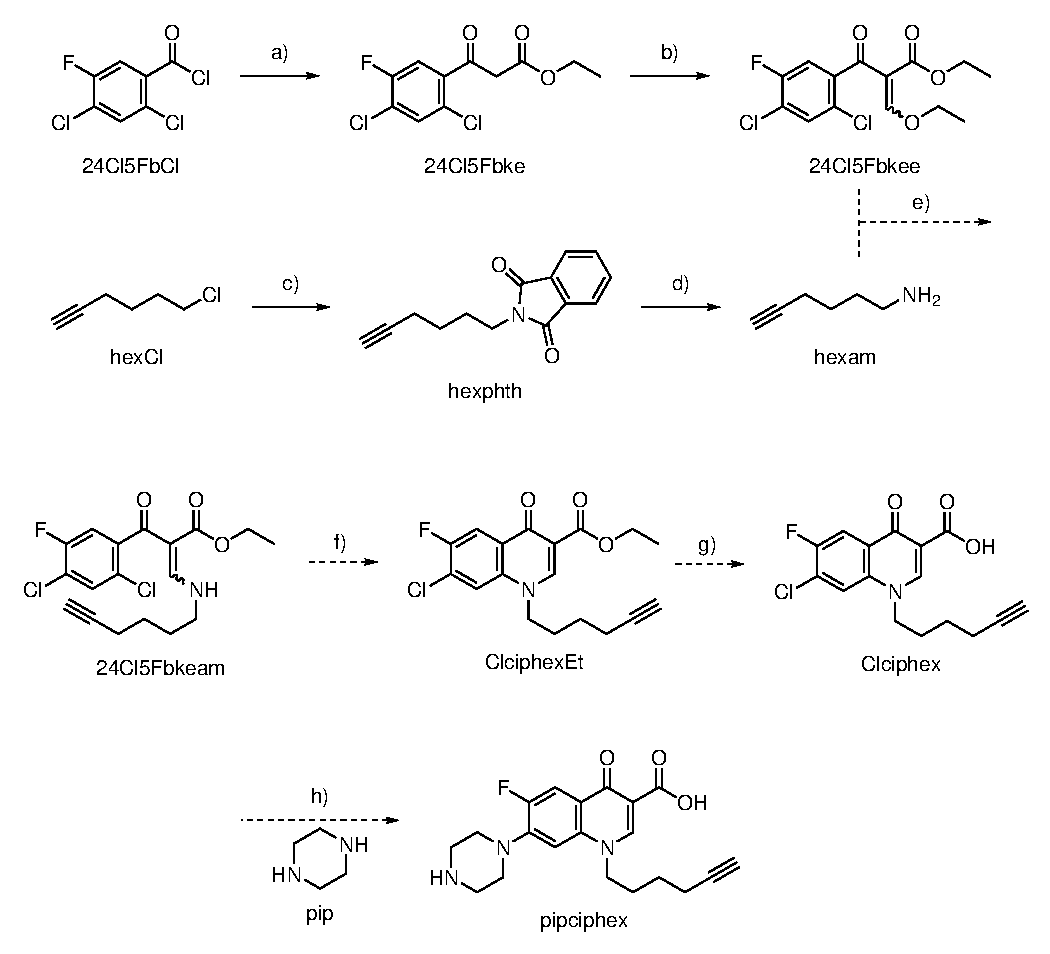
\includegraphics[scale=1]{pipciphex_synth}
		\caption{The synthesis of \compound{cmpd:pipciphex}.
		a) EtOAc, \ce{TiCl4}, DIPEA, \textit{N}-methyl imidazole, toluene, r.t., 30 min.
		b) Triethyl orthoformate, \ce{Ac2O}, reflux, 2 h.
		c) Potassium phthalimide, potassium iodide, DMF, 80 $^{\circ}$C, 18 h.
		d) \ce{N2H2.H2O}, EtOH, reflux, 18 h.
		e) EtOH.
		f) NaH, dioxane.
		g) KOH, THF.
		h) DMSO.
		\label{sch:pipciphex_synth}}
	\end{center}
\end{scheme}

\subsubsubsection{Sulfanilamide derivatives}

Sulfanilamide antibiotics were the first class of antibiotics to be widely used\cite{Otten1986,Wainwright2011}. They are all derivatives of 4-aminobenzenesulfonamide, very commonly with the sulfonamide nitrogen linking to a heterocycle. Sulfanilamide antibiotics function by inhibiting bacterial synthesis of folic acid. \textit{P. aeruginosa} has intrinsic resistance to sulfanilamides mainly due to the MexAB-OprM efflux pump\cite{Kohler1996} and so, as with trimethoprim \compound{cmpd:Tri}, it is hoped that conjugation to an autoinducer would restore activity.

Derivatives of 4-aminobenzenesulfonamide \compound{cmpd:Sul} have previously been synthesised using copper(I)-catalyzed alkyne-azide cycloaddition reactions to append various groups\cite{Wang2010} (see \ref{sch:Y1Sul_click}). However, if one considers sulfonamide antibiotics already in use, nearly all have a heterocycle linked directly to the sulfur atom, rather than with a methylene group in between. 

\begin{scheme}[H]
	\begin{center}
		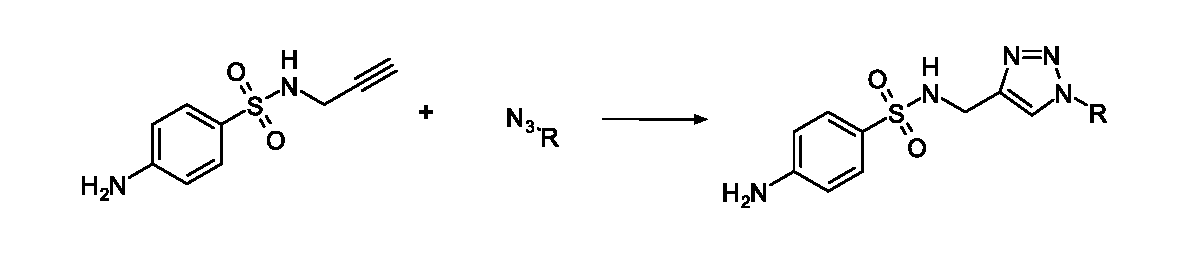
\includegraphics[scale=1]{Y1Sul_click}
		\caption{The sulfanilamide derivatives synthesised using click chemistry by Wang et al\cite{Wang2010}.
		\label{sch:Y1Sul_click}}
	\end{center}
\end{scheme}


Therefore, it was postulated that a 1,2,3-triazole could be introduced in the position occupied by a heterocycle in other known sulfonamide antibiotics by attachment of an alkyne directly to the sulfonamide nitrogen to form an alkynyl sulfanilamide derivative \compound{cmpd:Y0Sul} or a protected version of it (see \ref{sch:Y0Sul_idea}).

\begin{scheme}[H]
	\begin{center}
		\schemeref[Y0Sul]{cmpd:Y0Sul}
		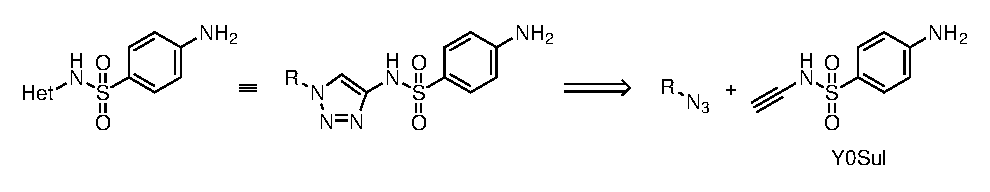
\includegraphics[scale=1]{Y0Sul_idea}
		\caption{Retrosynthesis of a 1,2,3-triazole-containing autoinducer-sulfonamide conjugate. R = autoinducer.
		\label{sch:Y0Sul_idea}}
	\end{center}
\end{scheme}

It was hoped that sulfanilamide derivative \compound{cmpd:Y0Sul} could be synthesised and reacted with the azido autoinducer derivatives directly. However, it appears that no secondary ynamides have been synthesised to date.
Conversely, the synthesis of tertiary ynamines has been studied more widely\cite{Ficini1976}. In particular, tertiary ynamides have been shown to be relatively stable and easy to work with in a variety of reactions including copper(I)-catalyzed alkyne-azide cycloadditions\cite{IJsselstijn2006,Evano2010}. 

The study of copper(I)-catalyzed alkyne-azide cycloadditions of ynamides by IJsselstijn et al.\cite{IJsselstijn2006} includes terminal ynamides protected using a benzyl and a tosyl group. Although their click reactions proceed with high yield, they do not present the deprotection of their final compounds. However, these reactions provided a promising suggestion that click reactions between a protected alkynyl sulfanilamide derivative and the azido autoinducer derivatives are feasible. The tosyl group used by IJsselstijn et al.\cite{IJsselstijn2006} to protect their ynamide is very similar to the \textit{p}-aminobenzenesulfonyl group needed in the alkynyl-sulfanilamide derivative. 
However, because installation of the alkyne could be problematic in the presence of a second amine, the \ce{NH2} group was installed as a \ce{NO2} group and reduced after the click reaction. 

The synthesis proceeded as shown in \ref{sch:HL2T0Sul_synth} \cite{Bendikov2005,Graux2014,IJsselstijn2006}. It was hoped that the methoxybenzyl group could be removed and the nitro group converted to an amine simultaneously by reduction in the last step, but unfortunately the methoxybenzyl group proved difficult to remove. On reflection, methoxybenzene was a poor choice of protecting group, and a more reduction-labile group such as benzyl or diphenylmethyl should have been chosen\cite{Wuts2007}.
This reaction could be repeated with a different choice of protecting group to provide another set of autoinducer-antibiotic conjugates.

\begin{scheme}[H]
	\begin{center}
	\schemeref[PMBa]{cmpd:PMBa}
	\schemeref[NsCl]{cmpd:NsCl}
	\schemeref[TIPSY]{cmpd:TIPSY}
	\schemeref[TIPSYBr]{cmpd:TIPSYBr}
	\schemeref[NsPMB]{cmpd:NsPMB}
	\schemeref[TIPSYNsPMB]{cmpd:TIPSYNsPMB}
	\schemeref[YNsPMB]{cmpd:YNsPMB}
	\schemeref[HL2N3]{cmpd:HL2N3}
	\schemeref[HL2TNsPMB]{cmpd:HL2TNsPMB}
	\schemeref[HL2T0Sul]{cmpd:HL2T0Sul}
		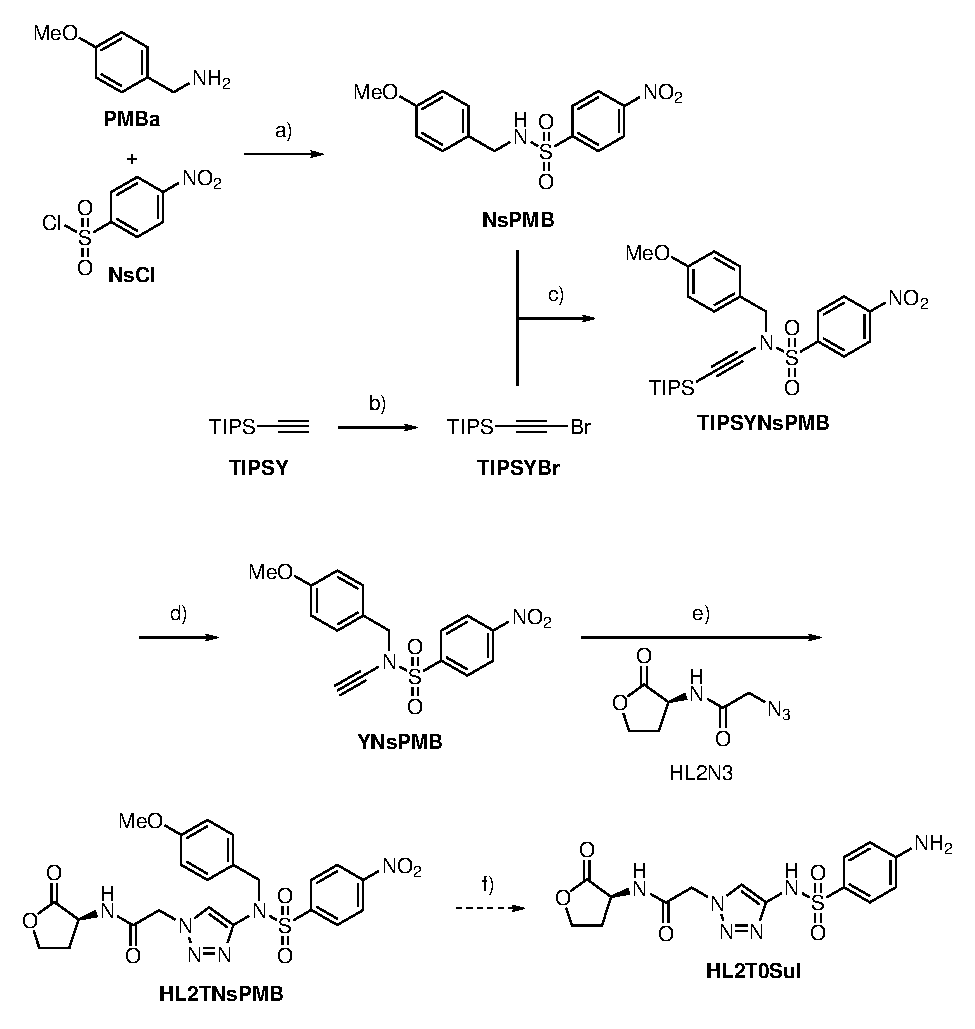
\includegraphics[scale=1]{HL2T0Sul_synth}
		\caption{Synthesis of a 1,2,3-triazole-containing sulfonamide antibiotic-autoinducer hybrid.
		a) \ce{CH2Cl2}, r.t., 24 h. 
		b) \ce{AgNO3}, acetone, r.t., 3 h. 
		c) \ce{CuSO4.5H2O}, 1,10-phenanthroline, \ce{K2CO3}, toluene, $80\ ^{\circ}$C, 48 h. 
		d) TBAF, THF, $-78\ ^{\circ}$C, 3 h. 
		e) \ce{Cu(OAc)2}, sodium ascorbate, \ce{CH2Cl2}, \textit{t}-BuOH, water, r.t., 16 h. 
		f) \ce{H2}, \ce{PtO2}, MeOH, 1 atm, r.t., 3 h.
		\label{sch:HL2T0Sul_synth}}
	\end{center}
\end{scheme}


\subsubsubsection{Linezolid derivative \compound{cmpd:Y4PipFOxaAmAc}}

Linezolid is a monoamine oxidase inhibitor used for the treatment of infections caused by Gram-positive bacteria.
Gram-negative bacteria, including \textit{P. aeruginosa} are resistant to linezolid due to the activity of efflux pumps, and hence it might be possible to increase its activity in such organisms by increasing its uptake and/or retention by conjugation to an autoinducer.

An alkynyl linezolid derivative \compound{cmpd:Lin} was partially synthesised by Ryan Howard (see \ref{sch:YLin_synth}). The route follows a procedure described by Phetsang \textit{et al}\cite{Phetsang2014} where the morpholine ring of linezolid is replaced by piperazine, allowing an alkynyl tail to be attached to the molecule.

The first three steps were carried out on a large scale, producing 55.7 g of \compound{cmpd:CbzPipFAmCbz}. As all steps except the final one are reported in the literature\cite{Phetsang2014,Khalaj2011} it is hoped that the alkynyl linezolid derivative \compound{cmpd:YLin} could be synthesised fairly straightforwardly.

\begin{scheme}[H]
	\begin{center}
		\schemeref[2FN]{cmpd:2FN}
		\schemeref[Pip]{cmpd:pip}
		\schemeref[PipFN]{cmpd:PipFN}
		\schemeref[PipFAm]{cmpd:PipFAm}
		\schemeref[CbzPipFAmCbz]{cmpd:CbzPipFAmCbz}
		\schemeref[RGlyBu]{cmpd:RGlyBu}
		\schemeref[CbzPipFOxaOH]{cmpd:CbzPipFOxaOH}
		\schemeref[CbzPipFOxaOTs]{cmpd:CbzPipFOxaOTs}
		\schemeref[KPhth]{cmpd:KPhth}
		\schemeref[CbzPipFOxaPhth]{cmpd:CbzPipFOxaPhth}
		\schemeref[CbzPipFOxaAm]{cmpd:CbzPipFOxaAm}
		\schemeref[CbzPipFOxaAmAc]{cmpd:CbzPipFOxaAmAc}
		\schemeref[PipFOxaAmAc]{cmpd:PipFOxaAmAc}
		\schemeref[Y4I]{cmpd:Y4I}
		\schemeref[Y4PipFOxaAmAc]{cmpd:Y4PipFOxaAmAc}
		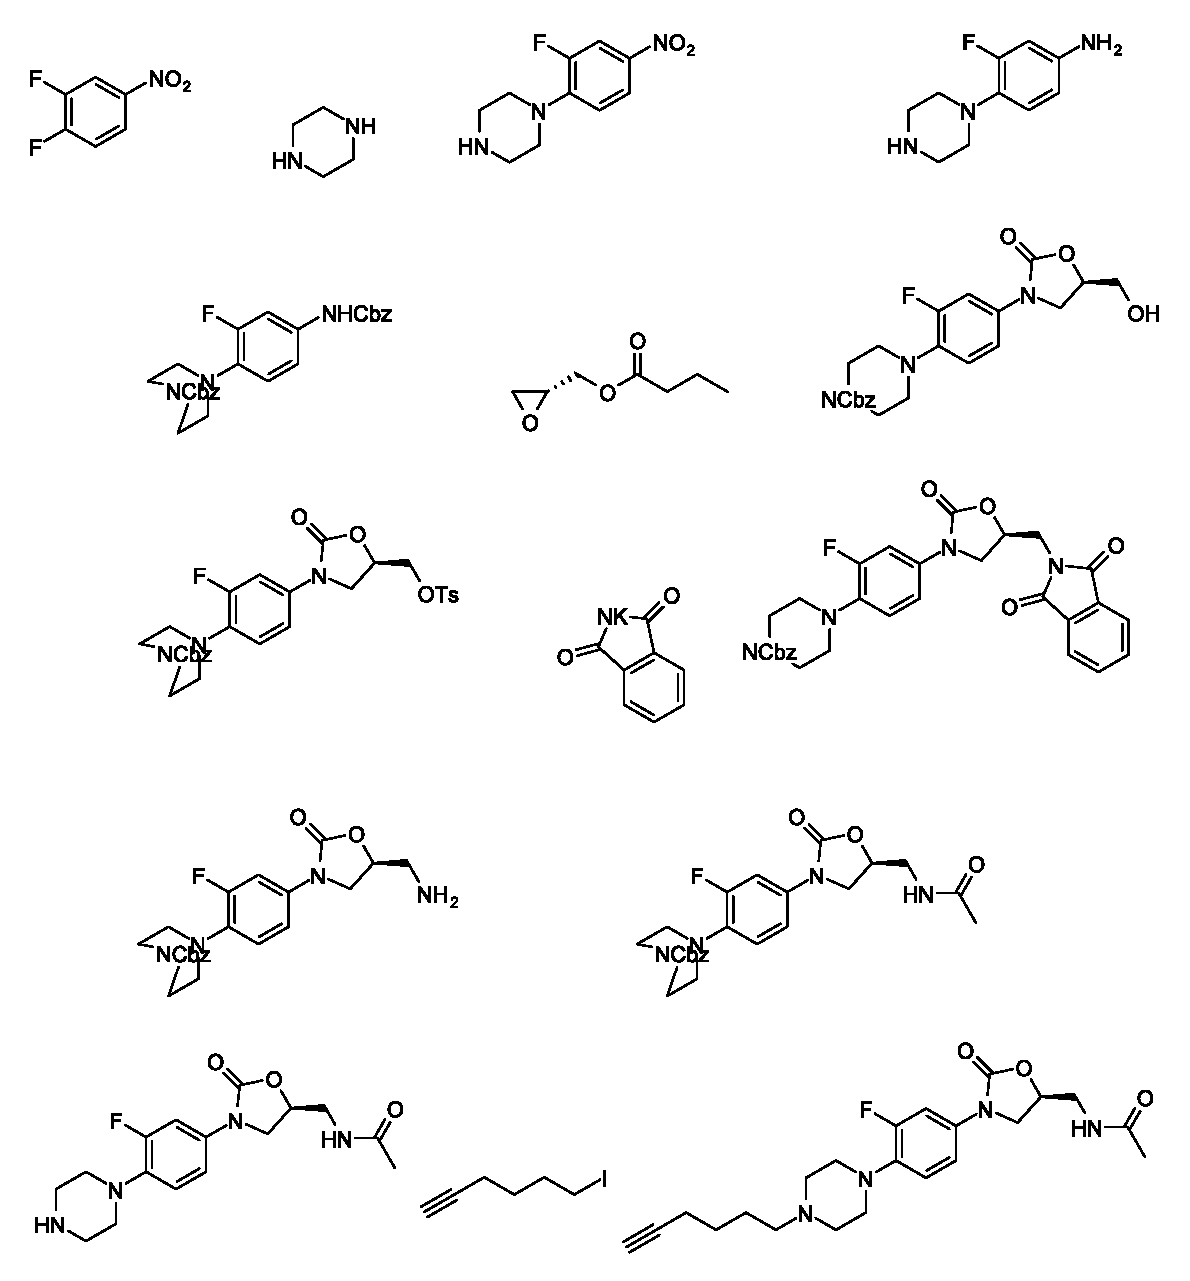
\includegraphics[scale=1]{YLin_synth}
		\caption{Proposed and partially completed synthesis of linezolid derivative \compound{cmpd:YLin}\cite{Phetsang2014}.
		a) MeCN, reflux, 3 h, 91\%. 
		b) \ce{H2}, 10\% Pd/C, THF, 40 psi, <50 $\ ^{\circ}$C, 1.5 h, 95\%. 
		c) CbzCl, \ce{Na2CO3}, acetone, water, 5 $\ ^{\circ}$C, 1 h then r.t., 16 h, 56\%. 
		d) \textit{n}-BuLi, THF, -78 $\ ^{\circ}$C, 1 h then add epoxide then -78 $\ ^{\circ}$C to r.t., 5 h. 
		e) TsCl, TEA, \ce{CH2Cl2}, 0 $\ ^{\circ}$C to r.t. 4.5 h. 
		f) Acetonitrile, water, reflux, 48 h. 
		g) \ce{MeNH2}, EtOH, water, reflux, 5.5 h. 
		h) \ce{Ac2O}, pyridine, 0 $\ ^{\circ}$C to r.t., 16 h. 
		i) \ce{H2}, 10\% Pd/C, MeOH/\ce{CH2Cl2}, 1 atm, r.t., 16 h. 
		j) \ce{NEt3}, EtOH, reflux.%, 6 h.
		\label{sch:YLin_synth}}
	\end{center}
\end{scheme}


\subsubsubsection{Gentamicin derivative \compound{cmpd:hexC1a}}

Gentamicin is an aminoglycoside antibiotic used to treat many bacterial infections, particularly those caused by Gram-negative organisms, by binding to the bacterial ribosome. Gentamicin is actually a mixture of components (see \ref{fgr:gen_anas}) synthesised by \textit{Micromonospora}, a genus of Gram-positive bacteria. Separation of the gentamicin components has been achieved by Grote \textit{et al.} \cite{Grote2012} by reaction with benzyl chloroformate followed by HPLC and hydrogenolysis of the protecting groups. 
Gentamicin C1a \compound{cmpd:C1a} was isolated pure, and is particularly useful because it the only component which contains a \ce{CH2NH2} group. This group is less hindered than all other amine groups in gentamicin C1a \compound{cmpd:C1a} and hence it is possible to selectively derivatise the molecule at this position. Grote \textit{et al.} attached a tag needed for an immunoassay using a pentafluorophenyl ester\cite{Cheshev2010}. Hence, it may be possible to achieve selective reaction of this site with the pentafluorophenyl ester of 5-hexynoic acid \compound{cmpd:hexOOpf} (see \ref{sch:hexC1a_synth}). It may even be possible to react the original gentamicin mixture with the pentafluorophenyl ester \compound{cmpd:hexOOpf} and then separate out the desired component.

\begin{figure}[H]
	\begin{center}
		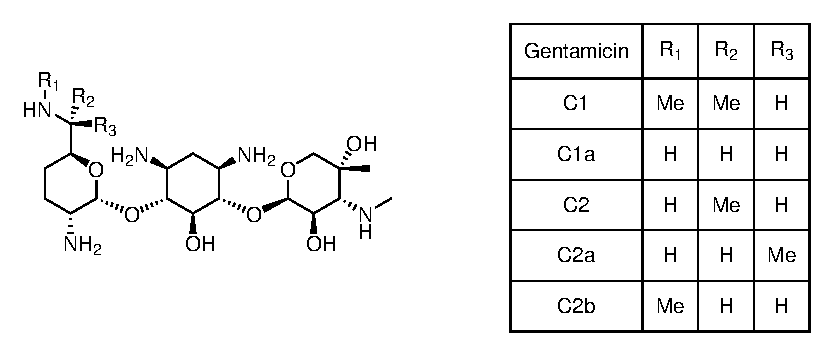
\includegraphics[scale=1]{gen_anas}
		\caption{Gentamicin components. \label{fgr:gen_anas}} 
	\end{center}
\end{figure}

\begin{scheme}[H]
	\begin{center}
		\schemeref[hexOOpf]{cmpd:hexOOpf}
		\schemeref[C1a]{cmpd:C1a}
		\schemeref[hexC1a]{cmpd:hexC1a}
		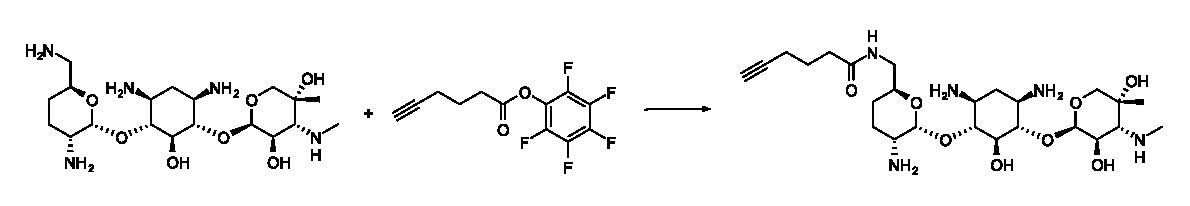
\includegraphics[scale=1]{hexC1a_synth}
		\caption{Proposed synthesis of gentamicin C1a derivative \compound{cmpd:hexC1a}. a) DIPEA, DMF, - 55 $^{\circ}$C. \label{sch:hexC1a_synth}}
	\end{center}
\end{scheme}

\subsubsubsection{Streptomycin derivative \compound{cmpd:redamalkyneNstr}}

Streptomycin \compound{cmpd:str} is an aminoglycoside antibiotic used to treat \textit{Mycobacterium tuberculosis} and \textit{S. aureus} which works by binding to the bacterial ribosome. There is limited SAR data on streptomycin but it is known that conversion of the aldehyde to a carboxylic acid destroys activity, whereas conversion to an alcohol retains it \cite{lemke2012foye}. 

Reductive amination can be used to install an alkyne group by reaction of the aldehyde with an amine such as oct-7-yn-1-amine \compound{cmpd:octam} (see \ref{sch:redamalkyneNstr_synth}). This approach has been used by Zhang \textit{et al.}\cite{Zhang2013} to form a conjugate of streptomycin \compound{cmpd:str} and chitosan which was active against biofilms. 
Reductive amination replaces the aldehyde O with NH; it is known that an OH is tolerated at this position so it makes sense that NH is as well.

\begin{scheme}[H]
	\begin{center}
		\schemeref[str]{cmpd:str}
		\schemeref[octam]{cmpd:octam}
		\schemeref[redamalkyneNstr]{cmpd:redamalkyneNstr}
		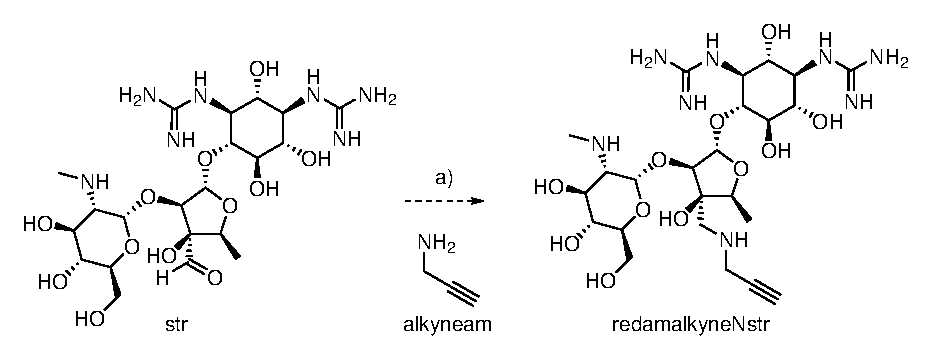
\includegraphics[scale=1]{redamalkyneNstr_synth}
		\caption{Proposed synthesis of streptomycin derivative \compound{cmpd:redamalkyneNstr}. 
		a) \ce{NaBH3CN}, water, r.t..
		\label{sch:redamalkyneNstr_synth}}
	\end{center}
\end{scheme}
